% =========================================================
% METODOLOGIA
% FINALIDADE: descrever o percurso da pesquisa, para que possa ser
%   compreendido e avaliado.
% ESCREVA: o que se aplica ao seu estudo (tipo de pesquisa, contexto,
%   participantes ou corpus, coleta, análise e aspectos éticos).
% CUIDADO: as subseções são sugestão; ajuste-as ao seu método.
% EXEMPLOS NESTE ARQUIVO: figura e quadro, com título, fonte e remissão.
% Imagens devem ser salvas na pasta 5-figuras/ (PDF, PNG ou JPG).
% =========================================================

\chapter{METODOLOGIA}
\label{cap:metodologia}

A metodologia descreve o percurso adotado para responder ao problema de pesquisa. O texto deve ser suficientemente detalhado para permitir a compreensão e a avaliação dos procedimentos, bem como sua eventual reprodução por outros pesquisadores.

\section{Caracterização da pesquisa}
\label{sec:caracterizacao}

% Natureza (básica ou aplicada), abordagem (qualitativa,
% quantitativa ou mista), objetivos (exploratória, descritiva
% ou explicativa) e procedimentos técnicos.
Nesta seção, caracteriza-se a pesquisa quanto à natureza, à abordagem do problema, aos objetivos e aos procedimentos técnicos, com fundamentação em autores da área. Quanto aos objetivos, por exemplo, \citeonline{gil2008} distingue as pesquisas exploratórias, descritivas e explicativas.

\section{Contexto e participantes}
\label{sec:participantes}

% Descreva o local, o período, a população, a amostra ou o
% corpus, com os critérios de inclusão e de exclusão.
Apresentam-se o local e o período de realização do estudo, a população ou o corpus investigado e os critérios de seleção dos participantes ou dos documentos, com indicação dos critérios de inclusão e de exclusão.

\section{Instrumentos e procedimentos de coleta de dados}
\label{sec:coleta}

Descrevem-se os instrumentos utilizados, como questionários, roteiros de entrevista, protocolos de observação ou bases de dados, e a forma como foram elaborados, validados e aplicados. Os instrumentos elaborados pelo(a) autor(a) podem ser apresentados em apêndice (Apêndice~\ref{apd:instrumento}).

A Figura~\ref{fig:etapas} ilustra o modo de inserir uma figura com título e fonte. O título é posicionado acima da imagem, e a fonte, logo abaixo, ambos alinhados às margens da ilustração.

% Exemplo de figura. Ajuste a largura em ilustracao{...}.
% Troque exemplo-figura.pdf pelo nome do seu arquivo (PDF, PNG ou JPG
% salvo em 5-figuras/), sem o nome da pasta.
% Figura de outra obra: \fonte{\citeonline[p.~10]{gil2008}.}
\begin{figure}[htbp]
\begin{ilustracao}{0.9\linewidth}
\caption{Etapas da pesquisa}
\label{fig:etapas}
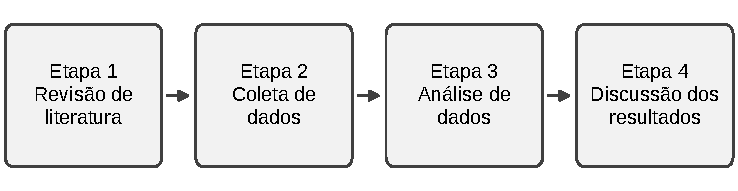
\includegraphics[width=\linewidth]{exemplo-figura.pdf}
\fonte{Elaboração própria (\ano).}
\end{ilustracao}
\end{figure}

\section{Procedimentos de análise dos dados}
\label{sec:analise}

% Indique as técnicas de análise (estatística descritiva ou
% inferencial, análise de conteúdo, análise do discurso etc.),
% os programas utilizados e as categorias de análise.
Explicitam-se as técnicas empregadas no tratamento e na análise dos dados, os programas computacionais utilizados, quando houver, e as categorias ou variáveis de análise. O Quadro~\ref{qua:procedimentos} exemplifica a relação entre objetivos específicos, procedimentos e instrumentos.

% Exemplo de quadro. Quadros têm bordas em todos os lados e
% apresentam informações textuais; dados numéricos devem ser
% apresentados em tabelas.
% Em cada linha, & separa as células e \\ \hline encerra a linha.
\begin{quadro}[htbp]
\centering
\caption{Relação entre objetivos específicos, procedimentos e instrumentos}
\label{qua:procedimentos}
\small
\begin{tabularx}{\linewidth}{|>{\raggedright\arraybackslash}X|>{\raggedright\arraybackslash}X|>{\raggedright\arraybackslash}X|}
\hline
\textbf{Objetivo específico} & \textbf{Procedimento} & \textbf{Instrumento} \\ \hline
Objetivo específico a & Procedimento de coleta ou de análise & Instrumento correspondente \\ \hline
Objetivo específico b & Procedimento de coleta ou de análise & Instrumento correspondente \\ \hline
Objetivo específico c & Procedimento de coleta ou de análise & Instrumento correspondente \\ \hline
\end{tabularx}
\fonte{Elaboração própria (\ano).}
\end{quadro}

\section{Aspectos éticos}
\label{sec:etica}

% Pesquisas com seres humanos devem ser aprovadas por Comitê de
% Ética em Pesquisa antes da coleta de dados. Informe o número
% do CAAE e do parecer.
Pesquisas que envolvem seres humanos devem ser submetidas à apreciação de Comitê de Ética em Pesquisa, por meio da Plataforma Brasil, antes do início da coleta de dados. Nas Ciências Humanas e Sociais, aplicam-se as disposições da Resolução nº 510/2016 do Conselho Nacional de Saúde \cite{brasil2016}. Informe o número do Certificado de Apresentação de Apreciação Ética (CAAE) e do parecer de aprovação, bem como os procedimentos adotados para obter o consentimento dos participantes e preservar o sigilo das informações.
